\documentclass[12pt,reqno]{amsart}
\usepackage{fullpage}
\usepackage{amsfonts}
\usepackage{tikz}
\usepackage{amssymb}
\usepackage{times}
\usepackage{graphicx}
\usepackage{mathtools}
\usepackage{breakurl}
\usepackage{bm}
\usepackage{blkarray}
\usepackage{url}
\usepackage[all]{xy}
\usepackage[margin=0.8in,footskip=0.25in]{geometry}

\usepackage[colorlinks=true,
            linkcolor=red,
            urlcolor=blue,
            citecolor=gray]{hyperref}
\vfuzz=2pt


\DeclarePairedDelimiter\ceil{\lceil}{\rceil}
\DeclarePairedDelimiter\floor{\lfloor}{\rfloor}

\DeclareMathOperator{\cok}{coker}
\DeclareMathOperator{\im}{im}
\DeclareMathOperator{\ann}{Ann}
\DeclareMathOperator{\Hom}{Hom}


% some "funny lines" referred to later:
\newtheorem{theorem}{Theorem}[section]
\newtheorem{corollary}[theorem]{Corollary}
\newtheorem{lemma}[theorem]{Lemma}
\newtheorem{proposition}[theorem]{Proposition}
{\theoremstyle{remark}\newtheorem*{remark}{Remark}}
\theoremstyle{definition}
\newtheorem{definition}[theorem]{Definition}
\newtheorem{example}[theorem]{Example}


\newcommand{\lex}{\mbox{lexdeg}}
\newcommand{\mymod}[3]{#1 \equiv #2 \Mod{#3}}
\newcommand{\ccc}{\mathcal{C}}
\newcommand{\nmm}[2]{\text{N}_{#1}(#2)}
\newcommand{\Mod}[1]{\ (\mathrm{mod}\ #1)}
\newcommand{\gal}{\text{Gal}}
\newcommand{\cc}{\mathbb{C}}
\newcommand{\zz}{\mathbb{Z}}
\newcommand{\ta}[1]{\langle #1 \rangle}
\newcommand{\ff}{\mathbb{F}}
\newcommand{\qq}{\mathbb{Q}}
\newcommand{\Tor}[2]{\mathbf{Tor}_{#1}(#2)}
\newcommand{\sqrtn}[1]{\sqrt[n]{#1}}
\newcommand{\charr}{\text{char}}
\newcommand{\disc}[1]{\mbox{disc}(#1)}
\newcommand{\Aut}{\text{Aut}}
\newcommand{\Inn}{\text{Inn}}
\newcommand{\Gal}{\text{Gal}}
\newcommand{\sgn}{\text{sgn}}
\newcommand{\irr}{\text{irr}}
\newcommand{\of}{\overline{F}}
\newcommand{\ok}{\overline{K}}
\newcommand{\ZZ}{\mathbb{Z}}
\newcommand{\NN}{\mathbb{N}}
\newcommand{\CC}{\mathbb{C}}
\newcommand{\QQ}{\mathbb{Q}}
\newcommand{\RR}{\mathbb{R}}
\newcommand{\FF}{\mathbb{F}}
\newcommand{\Tr}{\text{Tr}}
\newcommand{\nm}{\text{N}}
\newcommand{\tk}{\theta_K}
\newcommand{\mm}{\mathfrak{m}}
\newcommand{\tor}{\mathbf{Tor}}
\newcommand{\conv}[1]{\mathrm{conv}(#1)}
\newcommand{\diam}[1]{\mathrm{diam}(#1)}
\newcommand{\vol}[1]{\mathrm{vol}(#1)}
\newcommand{\la}{\langle}
\newcommand{\ra}{\rangle}

\begin{document}

\title{HW4}

\noindent \textbf{Q1:}

\begin{center}
  \begin{tikzpicture}[scale=3]
    \draw[very thick] (0,0) -- (2,0);
    \draw[very thick] (0,0) -- (1,1.732);
    \draw[very thick] (2,0) -- (1,1.732);
    \draw[very thick] (1,0) -- (1,1.732);
    \draw (0,0) -- (1.5, 0.866);
    \draw (2,0) -- (0.5, 0.866);
    \draw (0.5,0.866) -- (1.5, 0.866);
    \draw[dotted,thick] (0,0) -- (1, 0.866);
    \draw[dotted,thick] (2,0) -- (1, 0.866);
    \draw[dotted,thick] (1,0) -- (0.5, 0.866);
    \draw[dotted,thick] (1,0) -- (1.5, 0.866);
    \filldraw [red] (0,0) circle (1pt);
    \filldraw [red] (1,0) circle (1pt);
    \filldraw [red] (2,0) circle (1pt);
    \filldraw [red] (0.5, 0.866) circle (1pt);
    \filldraw [red] (1, 0.866) circle (1pt);
    \filldraw [red] (1.5, 0.866) circle (1pt);
    \filldraw [red] (1,1.732) circle (1pt);
    \filldraw [red] (1,0.57735) circle (1pt);
  \end{tikzpicture}
\end{center}


As indicated in the figure, the 8 points consist of 3 vertices of an equilateral triangle, 3 midpoints of edges, the mass center and the midpoint of the height. The 4 dotted lines are the ordinary lines.

\newpage
\noindent \textbf{Q2:} We borrow the ideas from graph theory. For each configuration $X$, we associate it with a matrix $m(X)$ with rows labeled by points and columns labeled by lines and with the entry value 1 if the point lies on the line and 0 if not. Relabeling and moving vertices around for a fixed configuration $X$ only permutes rows and columns of $m(X)$. In other words, if $X$ and $Y$ are two isomorphic combinatorial configurations, then there is a permutation matrix $P$ such that $m(Y)=P\cdot m(X)$. In particular, this means $m(X)$ and $m(Y)$ have the same rank.

Now label the Pappus configuration and another configuration as in the figure.

\begin{figure}[h]
  \centering
  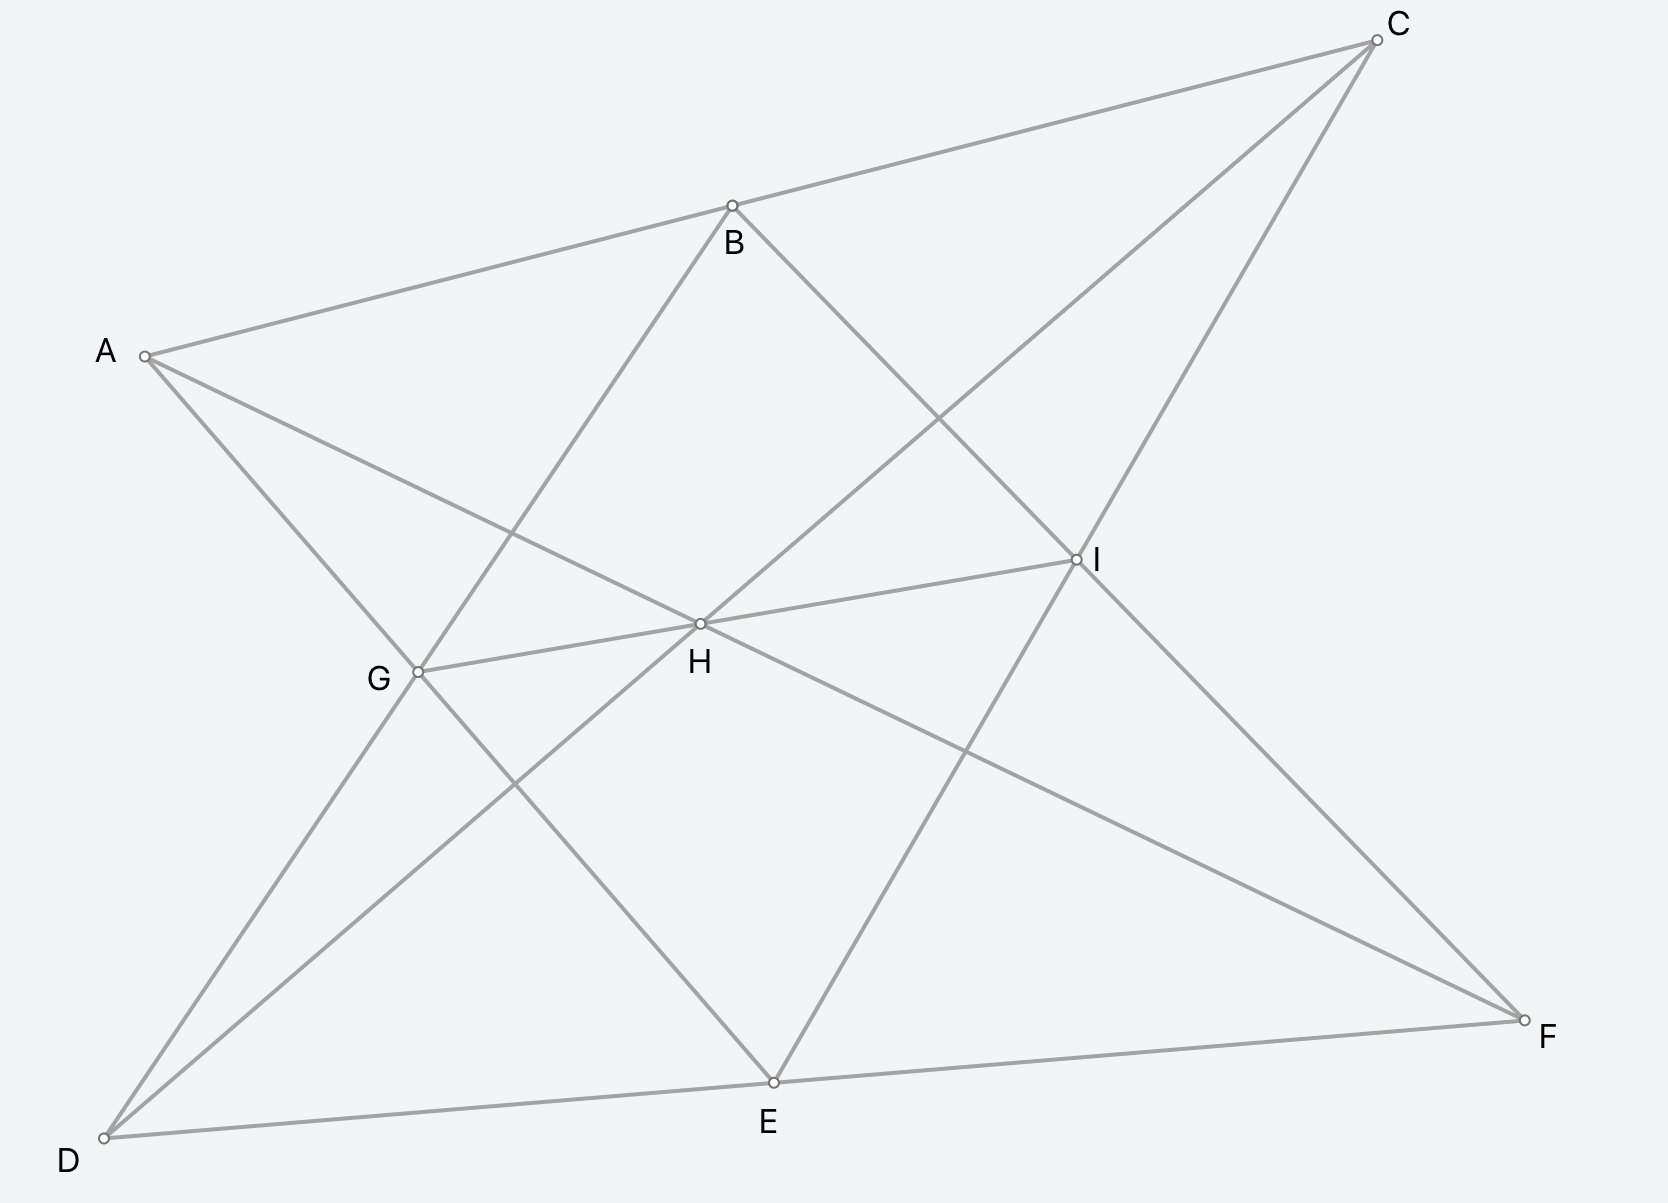
\includegraphics[width=8cm]{hw4a}
  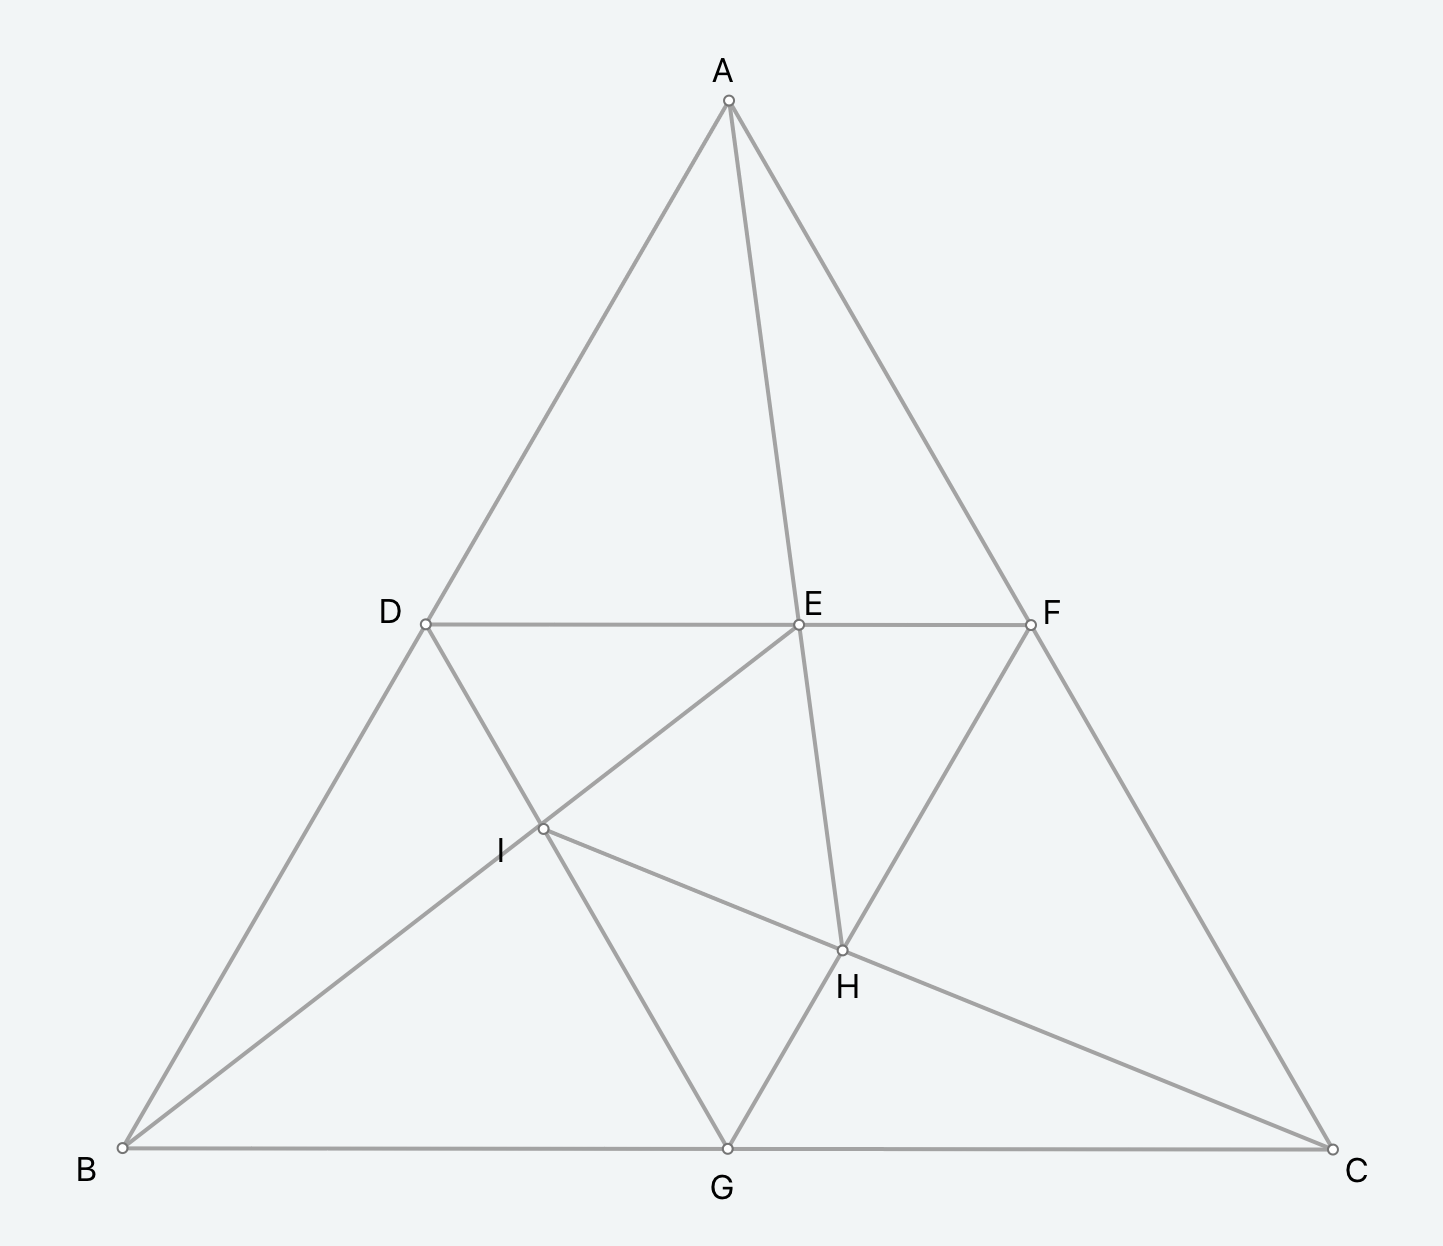
\includegraphics[width=7.5cm]{hw4b}
\end{figure}

Then the associated matrices are
\[
  \begin{blockarray}{cccccccccc}
    & ABC & AHF & AGE & BGD & BIF & CHD & CIE & GHI & DEF \\
    \begin{block}{c(ccccccccc)}
      A & 1 & 1 & 1 & 0 & 0 & 0&0&0&0 \\
      B & 1 & 0 & 0 & 1 & 1&0&0&0&0 \\
      C & 1&0&0&0&0&1&1&0&0\\
      D &0&0&0&1&0&1&0&0&1\\
      E &0&0&1&0&0&0&1&0&1\\
      F &0&1&0&0&1&0&0&0&1\\
      G &0&0&1&1&0&0&0&1&0\\
      H &0&1&0&0&0&1&0&1&0\\
      I &0&0&0&0&1&0&1&1&0\\
    \end{block}
  \end{blockarray} = m(X)
\]
and
\[
  \begin{blockarray}{cccccccccc}
    & ADB & AEH &AFC& BGC&BIE&CHI&DEF&DIG&GHF\\
    \begin{block}{c(ccccccccc)}
      A & 1 & 1 & 1 & 0 & 0 & 0&0&0&0 \\
      B & 1 & 0 & 0 & 1 & 1&0&0&0&0 \\
      C &0&0&1&1&0&1&0&0&0\\
      D &1&0&0&0&0&0&1&1&0\\
      E &0&1&0&0&1&0&1&0&0\\
      F &0&0&1&0&0&0&1&0&1\\
      G &0&0&0&1&0&0&0&1&1\\
      H &0&1&0&0&0&1&0&0&1\\
      I &0&0&0&0&1&1&0&1&0\\
    \end{block}
  \end{blockarray} = m(Y).
\]

But a straightforward calculation gives $\det(m(X)) = 0$ and $\det(m(Y))=27$. It follows that $m(X)$ and $m(Y)$ do not have the same rank and these two configurations are not isomorphic.


\newpage
\noindent \textbf{Q3:}

\begin{center}
  \begin{tikzpicture}[scale=1.5]
    \draw[very thick](0,0) circle (1);
    \draw[very thick](1.73205,0) circle (1);
    \draw[very thick](0.866,0.5) circle (1);
    \draw[very thick](0.866,1.5) circle (1);
    \filldraw [red] (0, 0) circle (1pt);
    \filldraw [red] (1.73205,0) circle (1pt);
    \filldraw [red] (0.866,0.5) circle (1pt);
    \filldraw [red] (0.866,1.5) circle (1pt);
  \end{tikzpicture}
\end{center}

As shown in the figure, the centers of the unit circles are $(0,0),(\sqrt{3},0),(\frac{\sqrt{3}}{2},\frac{1}{2})$ and $(\frac{\sqrt{3}}{2},\frac{3}{2})$.


\newpage
\noindent \textbf{Q4:} Let the $(q+1)$ points be $\{(1,x,x^2): x\in \FF_q)\}\cup\{ (0,0,1)\}$. We claim any three distinct points from these $(q+1)$ points are not collinear. These three points are either $(1,a,a^2),(1,b,b^2),(1,c,c^2)$ with $a,b,c\in \FF_q$ distinct or $(1,a,a^2),(1,b,b^2),(0,0,1)$ with $a,b\in \FF_q$ distinct. In either case, the claim follows from that \[ \det\begin{pmatrix}
    1 & a & a^2 \\
    1 & b & b^2 \\
    1 & c & c^2
  \end{pmatrix} =(c-a)(c-b)(b-a)\not= 0 \mbox{ and }  \det\begin{pmatrix}
    1 & a & a^2 \\
    1 & b & b^2 \\
    0 & 0 & 1
  \end{pmatrix} = b-a \not=0.\]
That no three points are collinear is to say every pair of points is contained in a unique line. So this is a complete $(n+1)$-point configuration.


\newpage
\noindent \textbf{Q5:} Let $A,B$ be two fixed points on the plane. Then $\triangle ABC$ is a triangle with area equal to 1 if and only  if $C$ lies on one of the two line which is at distance $\frac{2}{|AB|}$ form the line $AB$, because the area of a triangle is $\frac{1}{2}\mbox{base}\cdot\mbox{height}$. Now fix one point $X\in P$, then for any other point $Y\in P$, there are two lines as distance $\frac{2}{|XY|}$ from the line $XY$. These gives us at most $2(n-1)$ lines. In this point-line configuration, each triangle with area equal to 1 contributes to 1 incidence. By the Szemer{\' e}di-Trotter theorem, there are $O(n^{2/3}(2(n-1))^{2/3}+n^{2/3} +(2(n-1))^{2/3})=O(n^{4/3})$ incidences. That is, the number of unit-area triangles with a vertex at $X$ is at most $O(n^{4/3})$. Repeating the argument for all $X\in P$,  we conclude the maximum possible number of unit-area triangles is $O(n^{7/3})$.


\newpage
\noindent \textbf{Q6:} Let $n$ be the number of of distinct lines such that each of them contains at least $k$ points of $P$. Now by the Szemer{\' e}di-Trotter theorem, the maximum possible number of incidences is $O(m^{2/3}n^{2/3}+m+n)$. The trick here is that $O(m^{2/3}n^{2/3}+m+n)=\max\{O(m), O(n), O(m^{2/3}n^{2/3})\}$. Now each line gives at least $k$ incidences and so $$kn = O(m^{2/3}n^{2/3}) \quad\mbox{ or }\quad kn=O(m) \quad\mbox{ or }\quad km=O(m),$$ which gives us $$n=O(m^2/k^3) \quad\mbox{ or }\quad n=O(m/k) \quad\mbox{ or }\quad k=O(1).$$ But $k=O(1)$ gives no restrictions at all. Hence $m= O(m^2/k^3) +O(m/k)  = O(m^2/k^3+m/k)$\footnote{This is the upper bound given in Matou{\v{s}}ek's book.}, which of course is at most $O(m^2/k^2+m/k)$.


\newpage
\noindent \textbf{Q7:} Let us show the crossing number of the Petersen graph is 2. The figure\footnote{From \url{https://en.wikipedia.org/wiki/Petersen_graph}.} below shows the the crossing number is at most $2$.

\begin{figure}[h]
  \centering
  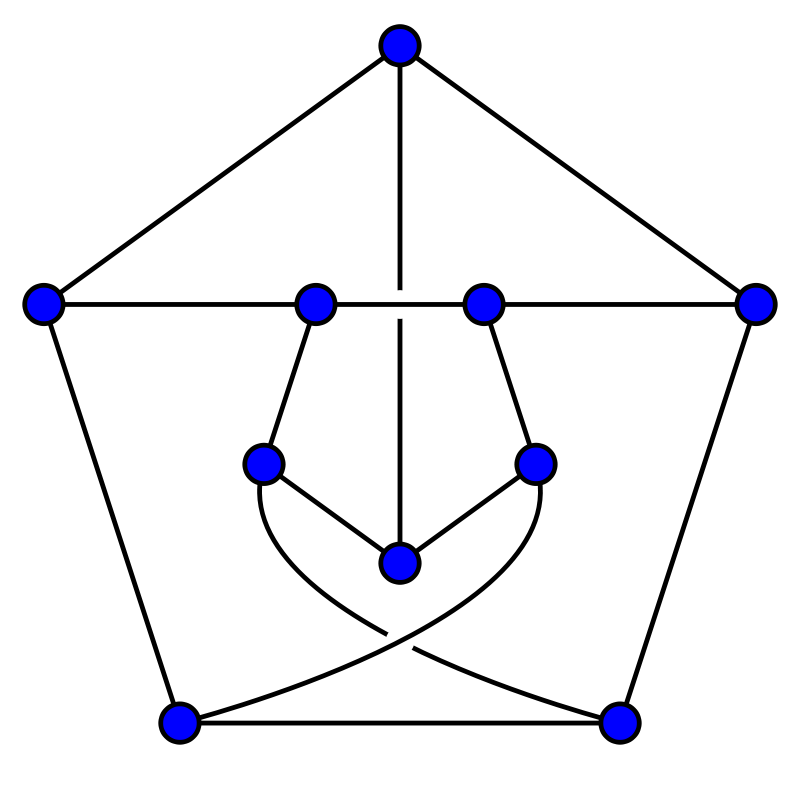
\includegraphics[width=4.5cm]{hw4c}
\end{figure}

The Petersen graph is symmetric, in particular, edge transitive. Suppose the Petersen graph can be drawn on the plane with one crossing or no crossing. Then with one edge removed, we get a planer graph. Since the Petersen graph is edge transitive, it implies the following graph, which is the the Petersen graph with one edge removed, is planer.

\begin{center}
  \begin{tikzpicture}[style=thick]
    \draw (18:2cm) -- (90:2cm) -- (162:2cm) -- (234:2cm) --
    (306:2cm);
    \draw (18:1cm) -- (162:1cm) -- (306:1cm) -- (90:1cm) --
    (234:1cm) -- cycle;
    \foreach \x in {18,90,162,234,306}{
        \draw (\x:1cm) -- (\x:2cm);
        \draw (\x:2cm) circle (2pt);
        \draw (\x:1cm) circle (2pt);
      }
    %\draw[ultra thick, red] (18:1cm) -- (18:2cm);
    % \draw[ultra thick, red] (90:1cm) circle (1pt);
    % \draw[ultra thick, blue] (162:1cm) circle (1pt);
    % \draw[ultra thick, red] (234:1cm) circle (1pt);
    % \draw[ultra thick, blue] (90:2cm) circle (1pt);
    % \draw[ultra thick, red] (162:2cm) circle (1pt);
    % \draw[ultra thick, blue] (234:2cm) circle (1pt);
  \end{tikzpicture}
\end{center}

But it contains a subgraph that is a subdivision of $K_{3,3}$ as shown below, contradicting to the Kuratowski's theorem. It follows that the Petersen graph has crossing number at least 2 hence is 2.

\begin{center}

  \begin{tikzpicture}[style=thick]
    \draw (18:2cm) -- (90:2cm) -- (162:2cm) -- (234:2cm) --
    (306:2cm);
    \draw (90:1cm) -- (306:1cm);
    \draw (18:1cm) -- (234:1cm);
    \draw (18:1cm) -- (162:1cm);
    \draw (162:1cm) -- (306:1cm);

    \foreach \x in {18,90,162,234,306}{
        \draw (\x:1cm) -- (\x:2cm);
      }
    %\draw[ultra thick, red] (18:1cm) -- (18:2cm);
    \draw[ultra thick, red] (18:1cm) circle (2pt);
    \draw[ultra thick, blue] (162:1cm) circle (2pt);
    \draw[ultra thick, red] (306:1cm) circle (2pt);
    \draw[ultra thick, blue] (90:2cm) circle (2pt);
    \draw[ultra thick, red] (162:2cm) circle (2pt);
    \draw[ultra thick, blue] (234:2cm) circle (2pt);
  \end{tikzpicture}
\end{center}


\end{document}


